%/*******************************************************************************
% * Copyright (c) 2007, G. Weirich
% * All rights reserved. This program may not be distributed
% * or modified without prior written consent
% *
% * Contributors:
% *    G. Weirich - initial implementation
% *
% *  $Id: anleitung.tex 291 2007-10-09 04:25:28Z Gerry $
% *******************************************************************************/

\documentclass[a4paper]{scrartcl}
\usepackage{german}
\usepackage[utf8]{inputenc}
\usepackage{makeidx}
\usepackage{wrapfig}
\makeindex
% Hier ein etwas skurriler Block, der dazu dient, die Unterschiede
% zwischen pdflatex und latex auszubügeln
% Grafiken müssen als png oder gif (für pdflatex) und als eps (für Latex)
% vorhanden sein. Die Endung kann man beim \includegraphics jeweils weglassen,
% das System nimmt je nach Renderer die geeignete Variante.

\newif\ifpdf
\ifx\pdfoutput\undefined
	\pdffalse              	%normales LaTeX wird ausgeführt
\else
	\pdfoutput=1
	\pdftrue               	%pdfLaTeX wird ausgeführt
\fi

\ifpdf
	\usepackage[pdftex]{graphicx}
	\DeclareGraphicsExtensions{.pdf,.jpg,.png}
\else
	\usepackage[dvips]{graphicx}
	\DeclareGraphicsExtensions{.eps}
\fi

\usepackage{floatflt}
\usepackage[]{hyperref}
\usepackage{color}
\title{Abrechnen mit Tarmed \& Co.}
\author{Gerry Weirich}

\begin{document}
\maketitle
\section{Einführung}
Der Weg vom Erbringen einer Leistung bis zum Einbuchen der Zahlung umfasst eine ganze Reihe verschiedener Schritte, die korrekt aufeinander abgestimmt werden müssen. Diese Broschüre erklärt die Konzepte und das Vorgehen beim Tarmed-System.

\medskip

Folgende Fragen müssen beantwortet werden, um korrekte Rechnungen zu erstellen und Zahlungen entgegenzunehmen\footnote{Dies ist nicht Elexis-spezifisch, sondern muss in jedem Praxisprogramm 'irgendwie' festgelegt werden. Bloss kann es bei weniger flexiblen Programmen 'festverdrahtet' sein, oder bei teuren Installationsveträgen kann die Konfiguration schon vom Hersteller vorgenommen werden sein. Da Elexis aber 'empowerment' des Anwenders auf den Fahnen stehen hat, müssen und dürfen Sie diese Dinge hier selber in die Hand nehmen (oder sich selber eine Supportfirma suchen, die es für Sie macht).}:

\begin{itemize}
\item Welches Tarifsystem und welche Tarifstufe wende ich an?
\item Für wen rechne ich ab?
\item An wen geht die Rechnung (und in welcher Form geht sie dorthin)?
\item Wer ist Kostenträger?
\item Wie identifiziere ich meine Leistungen gegenüber dem Kostenträger?
\item wohin sollen die Zahlungen gehen?
\item Woher weiss ich, ob Zahlungen eingegangen sind?
\item Wann und wie mahne ich?
\item Wann und wie leite ich Betreibungen ein?
\end{itemize}

Im Folgenden werde ich diese Schritte einzeln zeigen und die entsprechenden notwendigen Konfigurationen darlegen.

\section{Schritt für Schritt: Konfiguration}
Es sei an dieser Stelle nochmal darauf hingewiesen, dass diese Konfiguration nicht ganz trivial ist. Im Zweifelsfall sollten Sie es von einem Supporter durchführen lassen und stattdessen gleich im Abschnitt \ref{rechnungenerstellen} auf Seite \pageref{rechnungenerstellen} weiterlesen.

\medskip

\subsection{Abrechnungssysteme}
Die Leistungsverrechnung ist in Elexis als Plugin realisiert und damit auswechselbar oder auch ergänzbar - man kann nach Tarmed und nach CHOP, nach einem beliebigen Privatrechnungssystem und/oder nach einem österreichischen System abrechnen, das hängt nur davon ab, welche Plugins man installiert hat. Auch der Wechsel auf ein jetzt noch nicht bekanntes Tarifsystem ist damit kein Problem. Jedes Tarif-Plugin enthält das Codesystem selbst, sowie einen Mechanismus, um Rechnungen auszugeben, die zu diesem System konform sind (so muss eine Tarmed-Rechnung nicht nur andere Positionen beinhalten, sondern auch formal anders aussehen, als etwa eine Privatrechnung einer Heilpraktikerin). Ausserdem beinhaltet ein Abrechnungssystem je nachdem bestimmte ANgaben, die vorhanden sein müssen, um Rechnungen erstellen zu können (z.B. Kostenträger, Versicherungsnummer u. Ä.)


\medskip

Leistungscode, Ausgabeziel und erforderliche Daten, sowie die Tarifstufe sind in Elexis als 'Abrechnungssystem' zusammengefasst (S. Abb. \ref{fig:abr1}):
\begin{figure}
  % Requires \usepackage{graphicx}
  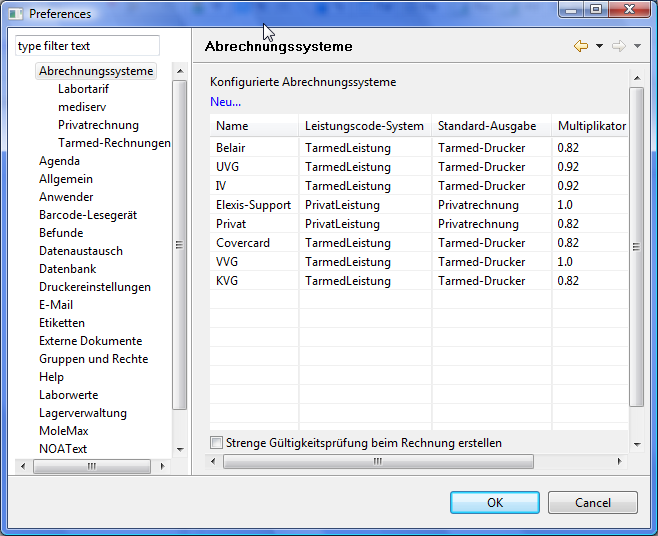
\includegraphics[width=0.9\textwidth]{abr1}\\
  \caption{Abrechnungssysteme: Übersicht}\label{fig:abr1}
\end{figure}
Es kann beliebig viele Abrechnungssysteme geben, und die Namen der einzelnen Abrechnungssysteme sind seitens Elexis egal. Um alle Schweizer Systeme abzudecken, sollten allerdings Abrechnungssysteme mit den Namen 'KVG', 'UVG', 'IV', 'MV' und 'VVG' vorhanden sein. Weitere können nach belieben dazukommen. Es ist beispielsweise problemlos möglich, zwei verschiedene KVG-Systeme mit verschiedenen Taxpunktwerten zu definieren.

\medskip

Um ein neues Abrechnungssystem zu erstellen, klickt man auf 'Neu...', um ein bestehendes zu modifizieren, klickt man doppelt darauf. Es öffnet sich der Abrechnungssystem-Konfigurationsdialog (Abb. \ref{fig:abr2}.
\begin{figure}
  % Requires \usepackage{graphicx}
  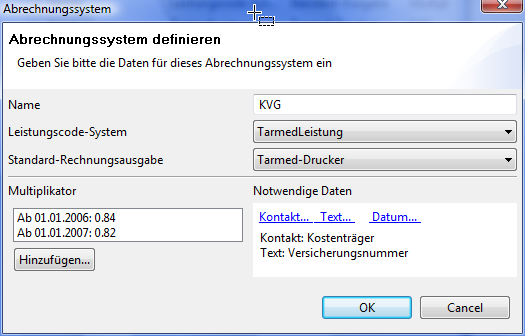
\includegraphics{abr2}\\
  \caption{KVG-Abrechnungssystem}\label{fig:abr2}
\end{figure}
Der Name ist wie gesagt frei wählbar. Für Leistungscode-System und Standard-Rechnungsausgabe können Sie aus den von den vorhandenen Abrechnungs-Plugins beigesteuerten Optionen wählen. Der Multiplikator ist die anzuwendende Tarifstufe (der 'Taxpunkt') für dieses System. Ein Multiplikator muss immer in Form einer Dezimalzahl angegeben werden und gilt immer ab einem bestimmten Datum so lange, bis ein anderer Multiplikator definiert wird. \textbf{Ein einmal eingegebener Multiplikator kann weder gelöscht noch geändert werden!}

Unter 'Notwendige Daten' geben Sie an, was für Angaben vorhanden sein müssen, damit ein Fall, der dieses Abrechnungssystem hat, als gültiog betrachtet wird. Solche Angaben können ein Kontakt sein, wie z.B. Kostenträger, oder ein Text, wie z.B. Versicherungs- oder Unfallnummer oder Vertragsnummer etc., oder es kann ein Datum sein, z.B. ein Unfalldatum.
Implizit immer notwendig ist der Kontakt 'Rechnungsempfänger', der deshalb hier nicht separat eingetragen werden darf.
Durch Rechtsklick kann man einen Eintrag in dieser Liste wieder löschen. Sie sehen das, was Sie hier eingegeben haben wieder unter den 'Fall-Details' als Fall-Erfordernisse (s. \ref{fall-erfordernisse}, S. \pageref{fall-erfordernisse}).

\subsection{Mandanten und Rechnungssteller}

Jeder Kontakt zwischen der Praxis und einem Patienten steht unter der Verantwortung eines \textit{Mandanten} und geht auf Rechnung eines \textit{Rechnungsstellers}. Im einfachsten und in der Schweiz üblichen Fall sind Mandant und Rechnungssteller identisch. Es ist aber auch möglich, dass ein Mandant im Fixlohn angestellt ist, auf eigen Verantwortung arbeitet, aber für einen anderen Rechnungssteller abrechnet (z.B. in einem HMO-Zentrum oder einer Polikinik). Dies ist nicht zu verwechseln mit einem Assistenten: Ein Assistent ist selber kein Mandant, sondern arbeitet auf Rechnung und unter der Verantwortung eines Mandanten. 

\medskip

Einen Mandanten erstellt man, indem man ihn unter den \textit{Kontakten} anlegt und das Häkchen 'Mandant' ankreuzt. Danach kann man unter \textsc{Datei-Einstellungen-Mandanten} Benutzername und Passwort eingeben und festlegen, für welchen REchnungssteller dieser Mandant arbeitet.

Diese Zusammenhänge sind auch im Elexis-Handbuch beschrieben, genaueres bitte ich dort nachzulesen.

\medksip

Zurück zum Tarmed-System: Wenn das Plugin 'elexis-arzttarife-schweiz' installiert ist, finden.


\section{Schritt für Schritt: Verrechnen, Rechnungen erstellen und ausgeben}
\label{rechnungenerstellen}
\label{fall-erfordernisse}
\end{document}
